\documentclass[conference]{IEEEtran}
\usepackage[T1]{fontenc}
\usepackage{graphicx}
\usepackage{booktabs}
\usepackage{array}
\usepackage{listings}
\usepackage{xcolor}
\usepackage{url}
\usepackage[hidelinks]{hyperref}
\graphicspath{{../docs/}}
\lstset{basicstyle=\ttfamily\scriptsize, breaklines=true, breakatwhitespace=false,
        columns=fullflexible, frame=single, framerule=0.3pt, rulecolor=\color{gray},
        xleftmargin=2pt, xrightmargin=2pt}
\newcommand{\code}[1]{\texttt{\small #1}}
\newcolumntype{L}[1]{>{\raggedright\arraybackslash}p{#1}}

\begin{document}

\title{One Workload, Four Engines: A Multi-Pipeline ETL and Reporting Framework for NASA Web
Server Logs on Pig, MapReduce, MongoDB and Hive}

\author{\IEEEauthorblockN{Sahiti (BT2024163) \quad Tushaar (BT2024022) \quad Aman (BT2024123) \quad Prajwal (BT2024245)}
\IEEEauthorblockA{\textit{DAS 839 NoSQL Systems, End-Semester Project, Final Report}\\
\url{https://github.com/sahiti3636/NoSQL_project}}}

\maketitle

\begin{abstract}
We built a tool that runs one fixed ETL and analytics workload over the NASA Kennedy Space Center
HTTP logs (July and August 1995, 3,461,613 lines) on a pipeline the user selects: Apache Pig,
MapReduce, MongoDB or Hive. Every pipeline parses the raw lines inside its own engine, computes
three queries per batch and for the whole run, and loads the results into PostgreSQL, where a
reporting module shows them with the run's runtime and batch statistics. A set of shared,
machine-readable \emph{contracts} keeps the four engines equivalent, and a row-by-row checker
proves it: at four batch sizes, including no batching, all four engines give identical answers
for every batch and for the whole run. The engines differ mainly in a fixed cost per batch:
about 0~s for MongoDB, 1.8~s for MapReduce, 8~s for Hive and 4.3~s for Pig. With large
batches MapReduce is fastest (51~s without batching); with small batches MongoDB is.
\end{abstract}

\section{Team and Work Division}
Each engine was built by two members: one took ingestion, parsing, malformed records and Q1, the
other the harder queries Q2 and Q3 and the whole-run results (Table~\ref{tab:team}).

\begin{table}[h]
\caption{Work division}
\label{tab:team}
\centering
\small
\begin{tabular}{@{}L{0.18\columnwidth}L{0.76\columnwidth}@{}}
\toprule
Member & Work \\
\midrule
Sahiti (A) & \textbf{MongoDB:} ingestion, parsing inside MongoDB, malformed records, Q1.
             \textbf{MapReduce:} \code{ParseJob}, \code{LogRecord}, Q1. Controller, batcher,
             loader; benchmark runs. \\
Tushaar (B) & \textbf{MongoDB:} Q2, Q3. \textbf{MapReduce:} Q2, Q3, whole-run counts, job
              settings. Equivalence checker, database tests. \\
Aman (C)   & \textbf{Hive:} RegexSerDe ingestion, HiveQL parsing, malformed records, Q1.
             \textbf{Pig:} ingestion, parsing in Pig Latin, malformed records, Q1. \\
Prajwal (D)& \textbf{Hive:} Q2, Q3, whole-run results. \textbf{Pig:} Q2, Q3, whole-run results.
             Reporting module. \\
\bottomrule
\end{tabular}
\end{table}

\section{Problem}
The input is the two official log files, unchanged except for decompression; the files are not
joined, cleaned or converted. Each line has a host, a timestamp, a quoted request, a status code
and a byte count. Every pipeline must extract host, timestamp, log date, log hour, HTTP method,
resource path, protocol version, status code and bytes (\code{-} means 0), count lines it cannot
parse, and compute:
\textbf{Q1}~requests and bytes per date and status;
\textbf{Q2}~the 20 most requested paths with bytes and distinct hosts;
\textbf{Q3}~errors (status 400--599), total requests, error rate and distinct error hosts per date
and hour. Input is processed in batches of N lines (IDs from 1, the last one may be short), the
runtime runs from the first byte read to the final database commit, and a report shows results with
pipeline, query, runtime, batch IDs, batch size and average batch size.

\section{Architecture}
Fig.~\ref{fig:arch} shows the design: one Python controller with four interchangeable engines
behind one interface (\code{prepare}, \code{process\_batch}, \code{finalize}, \code{cleanup}).

\begin{figure}[t]
\centering
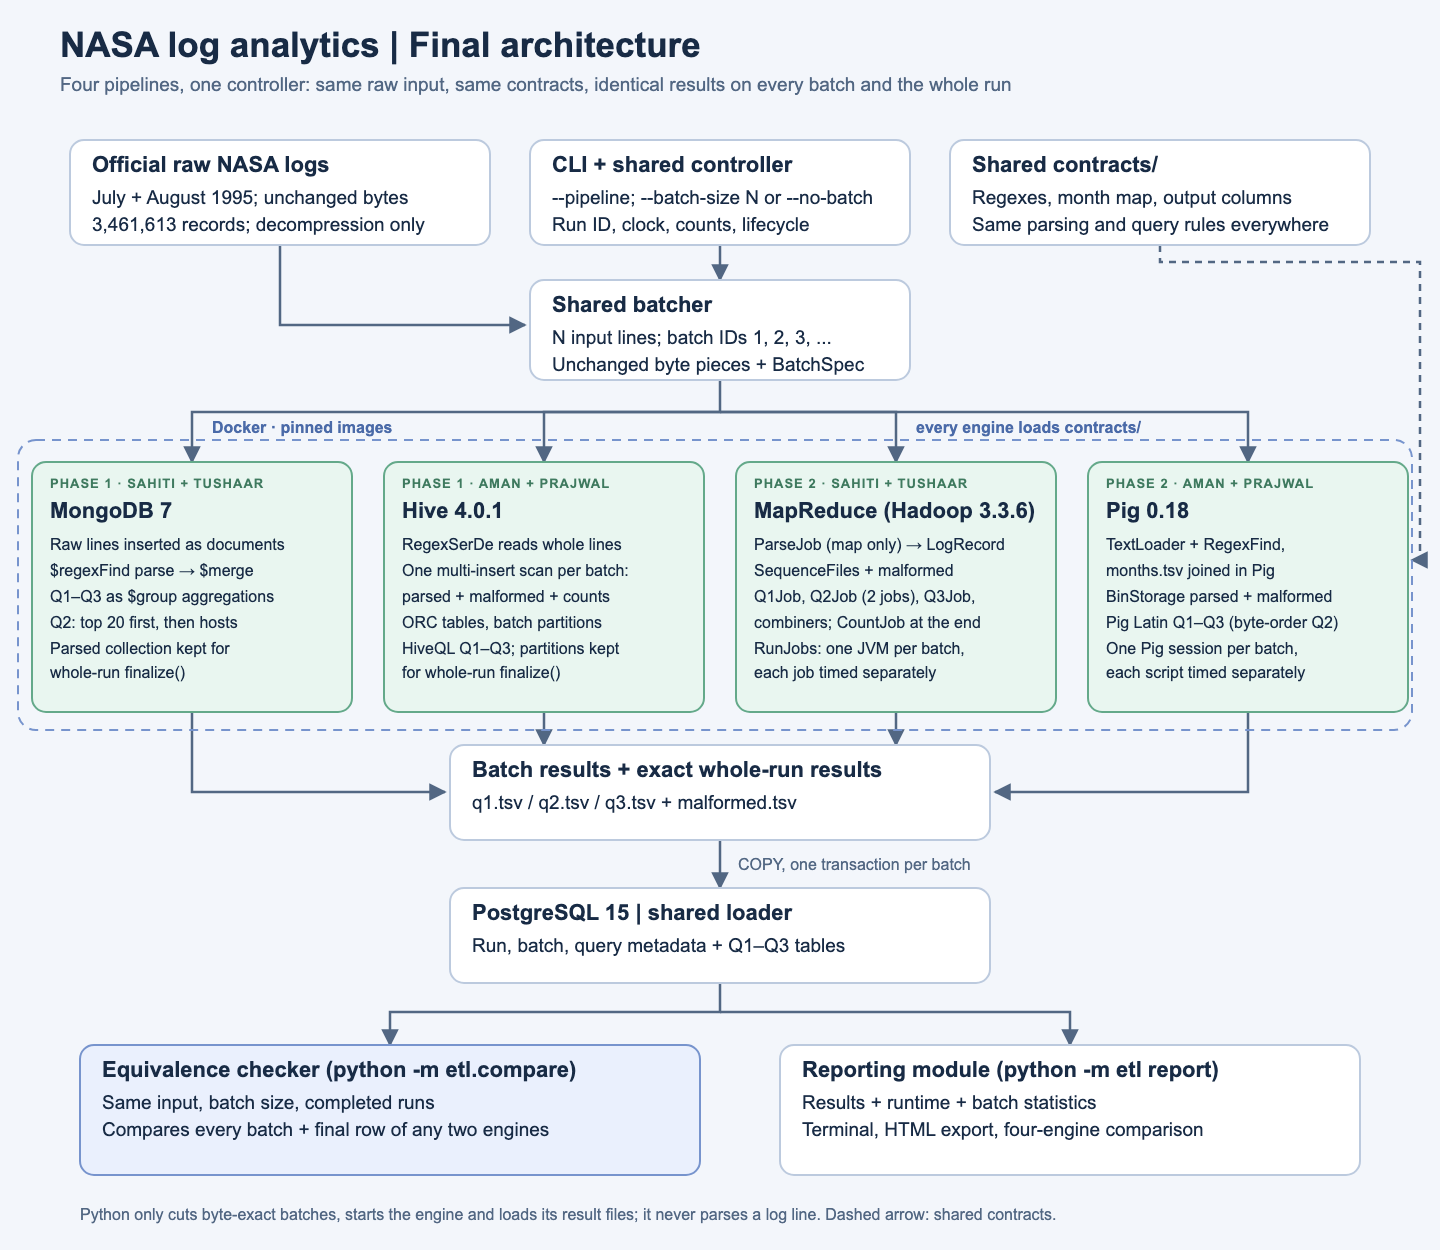
\includegraphics[width=\columnwidth]{architecture.png}
\caption{Final architecture. Python only cuts byte-exact batches, starts the engine and loads its
result files; all parsing and aggregation happen inside the selected engine.}
\label{fig:arch}
\end{figure}

\begin{itemize}
\item \textbf{CLI and controller} (\code{python -m etl run -{}-pipeline P -{}-batch-size N} or
  \code{-{}-no-batch}): creates the run, runs the clock, checks counts, handles failure.
\item \textbf{Contracts} (\code{contracts/}): the parsing regexes, the month map, the output
  columns and the controller--engine messages, loaded by every engine at run time.
\item \textbf{Engines}: MongoDB~7, Hive~4.0.1, MapReduce and Pig~0.18 on Hadoop~3.3.6, all in
  Docker with pinned images; Pig and MapReduce share one container.
\item \textbf{Loader and PostgreSQL~15}: one transaction per batch, constraints on every table.
\item \textbf{Report} (\code{python -m etl report}) and \textbf{checker}
  (\code{python -m etl.compare}) read only PostgreSQL.
\end{itemize}

\section{Parsing Approach}
Three regexes, stored as files and never retyped:
\begin{lstlisting}
envelope: ^([^ ]+) ([^ ]+) ([^ ]+) \[([0-9]{2})/([A-Za-z]{3})/([0-9]{4}):([0-9]{2}):([0-9]{2}):([0-9]{2}) ([+-][0-9]{4})\] "(.*)" ([0-9]{3}) ([0-9]+|-) *$
request:  ^ *([^ ]+) +(.*?)(?: +(HTTP/[0-9]+\.[0-9]+))? *$
fallback: ^ *(.*?) *$
\end{lstlisting}
Character classes are spelled out (\code{[0-9]}, not \code{\textbackslash d}) so Java, JavaScript
and Python read them alike. A line is \emph{malformed} when the envelope does not match or its
month is not in \code{months.tsv}; malformed lines are kept with their raw text and counted, never
dropped. The request regex splits method, path and protocol; when it fails, the fallback takes the
whole request as the path. \code{log\_date}, \code{log\_hour} and \code{log\_timestamp}
(\code{1995-07-01 00:00:01 -0400}) are sliced from the groups: date functions would convert time
zones (MongoDB's \code{\$dateFromString} shifts every hour by 4). Missing parts are \code{''},
never NULL; byte counts are 64-bit; invalid UTF-8 becomes U+FFFD, as Hadoop's \code{Text} does.

Edge cases found in the real data drove three rules: files are split on \code{\textbackslash n}
separately, because July ends with a truncated line (\code{alyssa.p}) that joining would hide;
seven request lines contain byte \code{0x01}, which breaks Hive's and Pig's default text formats;
and a lone \code{\textbackslash r} must not end a line, which Hadoop's default reader does.
A smoke test parses 2,038 such lines in every engine and compares every field with Python.

\section{ETL Workflow and Batching}
\begin{enumerate}
\item The controller records the run as \code{running} and calls \code{prepare()}.
\item The clock starts at the first byte read. The batcher copies exactly N lines into
  \code{runs/<run>/batch\_<id>/input} as unchanged byte pieces (a batch crossing from July to
  August has two pieces). This is slicing, not preprocessing: no field is read.
\item \code{process\_batch()} loads the lines into the engine, parses them there, keeps the parsed
  and malformed rows, and writes \code{q1.tsv}, \code{q2.tsv}, \code{q3.tsv} and
  \code{malformed.tsv} in PostgreSQL \code{COPY} text format.
\item The controller checks read = sent and valid + malformed = read, then the loader copies the
  batch's results in one transaction.
\item After the last batch, \code{finalize()} recomputes Q1--Q3 over \emph{all} kept parsed rows:
  summing per-batch distinct hosts or top-20 lists would be wrong.
\item The clock stops after the final commit; runtime, counts, number of batches and average batch
  size (= records / non-empty batches) are stored.
\end{enumerate}
\textbf{Failures:} any error rolls back the open transaction, marks the run \code{failed} with the
message and still cleans up the engine; reports show only successful runs, and a retry is a new run.
\textbf{No batching:} \code{-{}-no-batch} puts all 3,461,613 lines into batch~1, so each engine can
be measured without any per-batch cost.

\section{Pipeline Implementations}
\textbf{MongoDB.} Lines are inserted unparsed as \code{\{b, n, raw\}} documents; one aggregation
(\code{\$regexFind}, month lookup, typed fields) parses a batch and \code{\$merge}s it into a
parsed collection, which \code{finalize()} queries again. Q2 runs two aggregations: top 20 paths
first, then distinct hosts only over those 20 paths' rows. All queries use the simple (binary)
collation.

\textbf{Hive.} A \code{RegexSerDe} external table with \code{([\textbackslash s\textbackslash S]*)}
reads whole lines (the default format splits on \code{0x01}). One multi-insert scans each batch
once into ORC tables partitioned by batch (parsed, malformed) and a counts file. Q2 uses a CTE for
the top~20 and joins back for distinct hosts. One database per run.

\textbf{MapReduce.} A map-only \code{ParseJob} writes binary \code{LogRecord} SequenceFiles
(no delimiter can be safe with \code{0x01} and tabs in paths) and the malformed lines. \code{Q1Job}
and \code{Q3Job} use combiners; \code{Q2Job} runs a top-20 job then a hosts job for the 20
winners; \code{CountJob} counts whole-run records with \code{MultipleInputs}. \code{RunJobs} runs
all jobs of a batch in one JVM and times each.

\textbf{Pig.} \code{TextLoader} with \code{REGEX\_EXTRACT\_ALL('false')} (find semantics, like
Hive and Java), the month map joined from \code{months.tsv}, parsed and malformed rows kept with
\code{BinStorage}. One script parses and writes four outputs from a single scan; Q2 ranks all path
counts in one reducer by count and a byte-order key (a small Java UDF), then a replicated join
counts hosts for the 20. One Pig session runs a batch's four scripts.

\section{Query Implementation}
Table~\ref{tab:queries} compares the three queries across engines. All four follow the same plan
for Q2 (rank paths first, count distinct hosts only for the winners) and keep Q3 hours with zero
errors by grouping all rows and counting errors inside the group.

\begin{table}[h]
\caption{Query implementation per engine}
\label{tab:queries}
\centering
\scriptsize
\setlength{\tabcolsep}{3pt}
\begin{tabular}{@{}L{0.14\columnwidth}L{0.23\columnwidth}L{0.29\columnwidth}L{0.27\columnwidth}@{}}
\toprule
Engine & Q1 & Q2 & Q3 \\
\midrule
MongoDB & \texttt{\$group} (date, status) & \texttt{\$group} path, sort, limit; then \texttt{\$match \$in} + 2 groups & 2-stage \texttt{\$group} via (date, hour, host) \\
Hive & \texttt{GROUP BY} & CTE top 20, join, \texttt{count(DISTINCT)} & \texttt{sum(if)}, \texttt{count(DISTINCT if)} \\
MapReduce & combiner sums (1, bytes) & top-20 heap job, hosts job & mergeable partial with host set \\
Pig & \texttt{GROUP}, \texttt{COUNT\_STAR} & nested \texttt{ORDER}/\texttt{LIMIT}, replicated join & nested \texttt{FILTER} + \texttt{DISTINCT} \\
\bottomrule
\end{tabular}
\end{table}

Q2 ties are broken by the path in UTF-8 byte order everywhere (PostgreSQL \code{COLLATE "C"},
Hadoop \code{Text}, MongoDB simple collation, Pig UDF), because Java and Pig string comparison
orders characters above U+FFFF differently; a test with 21 tied paths checks the cut-off.

\section{Result Schema}
PostgreSQL schema \code{etl} (\code{sql/schema.sql}):
\begin{itemize}
\item \code{etl\_run}: pipeline, batch size, status, start/finish, runtime, total/valid/malformed
  records, batches, average batch size (generated column), input hash and manifest.
\item \code{etl\_batch}: batch ID, line range, counts, source pieces, time.
\item \code{query\_def}, \code{query\_execution}: per query and batch (and whole run): time, row
  count, SHA-256 fingerprint of the sorted rows.
\item \code{q1\_daily\_traffic}, \code{q2\_top\_resources}, \code{q3\_hourly\_errors},
  \code{malformed\_record}: every row carries pipeline, run ID, batch ID (NULL = whole run) and
  execution time, as the brief requires.
\end{itemize}
Constraints reject inconsistent data (valid + malformed = total; error rate = errors / total;
one whole-run result set per run via \code{UNIQUE NULLS NOT DISTINCT}). Views feed the report and
the comparison (\code{v\_run\_report}, \code{v\_q2\_final} with SQL ranking,
\code{v\_pipeline\_comparison}, \code{v\_equivalence}).

\section{Correctness and Equivalence}
A plain Python implementation is the answer key. Every run is checked three ways:
\begin{itemize}
\item \code{verify\_reference.py}: final rows and fingerprints equal the answer key
  (Q1 295, Q2 20, Q3 1,369 rows).
\item \code{etl.compare}: same input hash and batch boundaries, then a full outer join of every
  Q1--Q3 row of every batch and of the whole run, plus the malformed lines; error rates within
  $10^{-12}$.
\item \code{v\_equivalence}: number of distinct fingerprints per query across engines.
\end{itemize}
All 16 final runs (4 engines $\times$ 100k, 500k, 1M, no batching) read 3,461,613 records with
1 malformed line, pass the answer-key check, and are \textbf{equivalent} to MongoDB at the same
batch size; each query has exactly one distinct answer at every batch size. Field-level checks
(all nine parsed fields, timestamp included) cover every parsed MongoDB document, Hive's parsed
table on the smoke sample, and Pig's and MapReduce's parsed records on the smoke sample plus made-up
edge cases (tab and backslash in a top path, tied ranks, unknown month, trailing \code{\textbackslash r}).

\section{Experiments}
All runs: one laptop (Apple M3 Pro, Docker with 8~GB, mains power), the full input, one run per
configuration, nothing else running (Table~\ref{tab:runtime}, Fig.~\ref{fig:bench}).

\begin{table}[h]
\caption{Full-run runtime (s), first byte read to final commit}
\label{tab:runtime}
\centering
\small
\begin{tabular}{@{}lrrrrr@{}}
\toprule
Batch size & Batches & MongoDB & Hive & MapReduce & Pig \\
\midrule
100,000 & 35 & \textbf{97.2} & 425.1 & 111.7 & 261.4 \\
500,000 & 7 & 94.8 & 207.2 & \textbf{65.6} & 137.1 \\
1,000,000 & 4 & 99.8 & 171.4 & \textbf{56.6} & 128.9 \\
none & 1 & 97.1 & 149.3 & \textbf{51.2} & 114.3 \\
\bottomrule
\end{tabular}
\end{table}

\begin{figure}[t]
\centering
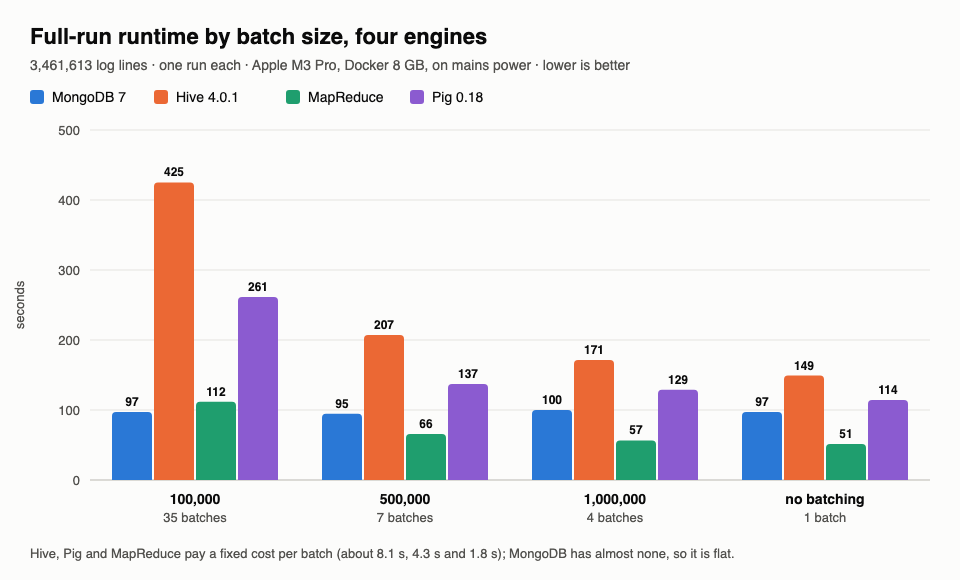
\includegraphics[width=\columnwidth]{benchmark_runtime.png}
\caption{Runtime by batch size. MongoDB is flat; the Hadoop-based engines pay per batch.}
\label{fig:bench}
\end{figure}

\textbf{Fixed cost per batch.} Fitting runtime against the number of batches gives a per-batch
cost of $\approx$0~s for MongoDB, 1.8~s for MapReduce, 8.1~s for Hive and 4.3~s for Pig.
Hive, Pig and MapReduce start jobs for every batch (Hive compiles four scripts into Tez work, Pig
compiles each script into Hadoop jobs); MongoDB's aggregations run in a server that is already up.

\textbf{Work.} Without batching, MapReduce is fastest (51~s): one map-only parse scan, combiners
before every shuffle and binary records read back without re-parsing. MongoDB (97~s) is limited by
inserting 3.46M documents, Pig (114.3~s) and Hive (149~s) by planning overhead and their
general-purpose operators.

\textbf{Measured improvements} (same laptop, 500k): \code{RunJobs} (one JVM per batch) cut
MapReduce from 72.9~s to 65.6~s; one Pig session per batch, 100~ms job polling and a top-20 step
without a sampling job cut Pig from 187.8~s to 137.1~s; ranking paths before counting hosts cut
MongoDB's whole-run Q2 from 11.2~s to 6.5~s. Earlier, Hadoop's 5~s job-completion poll had left
every MapReduce batch idle for up to 25~s.

\textbf{Lesson on measurement.} A first attempt ran with macOS Low Power Mode on and stray
background processes using about 8 cores; engines were 1.5--10$\times$ slower and those runs were
discarded. A Docker health check that started three JVMs every 15~s also took CPU from the timed
engine and was replaced by a check that starts none.

\section{Comparison of the Four Pipelines}
\begin{table}[h]
\caption{Summary comparison}
\label{tab:compare}
\centering
\scriptsize
\setlength{\tabcolsep}{3pt}
\begin{tabular}{@{}L{0.15\columnwidth}L{0.19\columnwidth}L{0.18\columnwidth}L{0.19\columnwidth}L{0.19\columnwidth}@{}}
\toprule
 & MongoDB & Hive & MapReduce & Pig \\
\midrule
Correctness & equivalent & equivalent & equivalent & equivalent \\
Runtime & flat $\approx$97~s; best for small batches & slowest at small batches; 8.1~s per batch & fastest with large batches (51~s) & 4.3~s per batch; 114~s unbatched \\
Difficulty & medium: aggregation pipelines, collation & medium: SerDe, ORC, escaping & highest: Java jobs, Writables, job chains & medium: escaping, \texttt{BinStorage}, ordering \\
Suitability & interactive, incremental loads & SQL users, large batch reports & large, fixed, performance-critical jobs & quick dataflow scripts over raw files \\
\bottomrule
\end{tabular}
\end{table}

\textbf{Correctness} was equal by construction: the shared contracts and the checker found no
difference anywhere. \textbf{Difficulty} differed most in the details: every Hadoop-based engine
needed binary storage for the parsed rows, an escape step for PostgreSQL, and care with line
endings and string ordering; MapReduce needed the most code. \textbf{Suitability for
semi-structured logs:} MongoDB suits small, frequent batches and ad-hoc questions; Hive suits SQL
users and large periodic batches; MapReduce gives the best throughput for a fixed workload at the
cost of code; Pig is the quickest to write for dataflow over raw text.

\section{Limitations}
Every engine runs in local mode in one container on one laptop, not on a cluster; absolute times
would differ elsewhere, the per-batch shape is the finding. Final timings are one run per
configuration (Phase~1 had three rounds for MongoDB and Hive, with similar spread). MongoDB needs
Python to decode and insert the raw lines, as the database stores only valid UTF-8 documents.

\section{Reproduction}
\begin{lstlisting}
docker compose -f docker-compose.yml -f compose.lock.yml up -d --build --wait
python -m etl run --pipeline pig --batch-size 500000
python -m etl run --pipeline pig --no-batch
python -m etl report --pipeline pig --html pig.html
python -m etl report --compare
python -m etl.compare --left-run A --right-run B
ROUNDS=1 ./scripts/run_benchmarks.sh
\end{lstlisting}

\begin{thebibliography}{6}
\bibitem{nasa} Internet Traffic Archive, ``NASA-HTTP,'' \url{https://ita.ee.lbl.gov/html/contrib/NASA-HTTP.html}.
\bibitem{mongo} MongoDB, ``Aggregation pipeline,'' \url{https://www.mongodb.com/docs/v7.0/aggregation/}.
\bibitem{hive} Apache Hive, ``LanguageManual DDL: RegexSerDe and ORC,'' \url{https://cwiki.apache.org/confluence/display/Hive/LanguageManual+DDL}.
\bibitem{hadoop} Apache Hadoop 3.3.6, ``MapReduce tutorial,'' \url{https://hadoop.apache.org/docs/r3.3.6/hadoop-mapreduce-client/hadoop-mapreduce-client-core/MapReduceTutorial.html}.
\bibitem{pig} Apache Pig 0.18, ``Pig Latin basics,'' \url{https://pig.apache.org/docs/latest/basic.html}.
\bibitem{pg} PostgreSQL 15, ``COPY,'' \url{https://www.postgresql.org/docs/15/sql-copy.html}.
\end{thebibliography}

\end{document}
